\chapter{Al'Anfanische Prophezeiungen}

\textbf{Einleitung}

Wohl erzittert der Sterbliche, wenn sich der Kelch der Katastrophe über ihn ergießt, doch wisse, dass die Ungaben der Unsterblichen oft zwiefach sind.

\textbf{I. Spruch: Von der Zweiheit der göttlichen Ungaben}

Zweimal, nicht einmal wird der Zwist der Zwillingsbrüder offenbar, und der Geber der Gestalt unterliegt, damit der Nehmer der Welt unterliegen muß.\\
Zweimal, nicht einmal werden die tumben Söhne Ogerons dem Kreuz des Nordens folgen.\\
Zweimal, nicht einmal werden die Botschafter von Ordnung und Einheit zweiteilen Ordnung und Einheit.\\
Zweimal, nicht einmal werden die Legionen des Roten Mondes vor das Haus der Gelben Sonne treten.\\
Zweimal, nicht einmal wird der Rabe nach dem Thron des Herren über Zwölf greifen.

\textbf{II. Spruch: Von Drachen und Kaisern}

Wenn sich Drachenblut mit Menschenblut auf einem Berg von Gold verbindet.\\
Wenn sich wegen des Schicksals der Zwillingskaiser nicht erfüllen kann das Schicksal der Kaiserzwillinge.\\
Wenn der alte Elfenkönig und der neue Elfenkönig mit Schiff und Roß heimgekehrt und bewiesen, dass der Elfenkönig nimmermehr wahr.\\
Wenn der alte Kaiser dem neuen Kaiser nachfolgt.\\
Wenn in der Neunflüssigen ein Alter Drache bar eines Karfunkels und ein Alter Karfunkel bar eines Drachen weilen.

\textbf{III. Spruch: Von den Handlangern des Untergangs}

Wenn der Diener jenseits des Todes den Meister außerhalb des Todes ruft.\\
Wenn die Verderberin der Leiber einen Leib dem Verderber der Welten verschafft.\\
Wenn die verlorenen Scharen der Gestaltlosen annehmen die Gestalt der Schar der Verlorenen.\\
Wenn aus kristallenem Herz der geraubte Schlangenfürst spricht.\\
Wenn die Bäume auf der See wurzeln, die Festungen über Land wandeln, und die Belagerungstürme über den Himmel ziehen.

\textbf{IV. Spruch: Von den sieben Gezeichneten}

Wenn der alleine Ahnende mit dem almadinen Auge angekommen.\\
Wenn der Bote des wandelnden Bildes zum Bündnis bittet.\\
Wenn das kühne Tier mit dem Krötensinn seinen Kürschmeister gekürt.\\
Wenn fünf firnglänzende Finger den Fluch der Felder gefunden.\\
Wenn nur mehr die stählerne Stirn den schrecklichen Schatten standhält.\\
Wenn das geflügelte Geschoß dem Grauen der Götter gilt.\\
Wenn aus sieben Schalen Schärfe schäumt, dagegen kein Schrecknis gewachsen ist.

\textbf{V. Spruch: Vom Ende des Zeitalters}

Dann wird in den Kerker der feurige Blick des Weltenschöpfers fallen.\\
Dann wird die rote Saat der Gor aufgehen.\\
Dann wird die letzte Kreatur geboren und gebären.\\
Dann werden Löwin und Einhorn zu Zweien ins Tal der Finsternis gehen.\\
Dann werden die Wasser blutig und die Brunnen sauer, der Regen brennend und das Land schimmelig.\\
Dann wird die Brut den Boden verschlingen.\\
Dann wird der Rausch der Ewigkeit über die Schöpfung wehen.


\section{Die Orakelsprüche von Fasar (vollständig)}

Dies ist die Kunde von den Zeiten da sich das Angesicht der Welt wandeln wird

\textbf{Spruch I}

\begin{enumerate}
    \item Wenn der Drache seinen Karfunkelstein verliert, wird sich die Kunde verbreiten von SEINER künftigen Macht und SEIN Diener stirbt und kann doch nicht sterben.
    \item Wenn der Sohn des Raben von der Tochter der Schlange niedergestreckt wird, erhebt sich wieder das leuchtende Zelt, und der Herrscher des Zeltes wird sein der dritte seines Namens.
    \item Wenn der Kaiser aus Borons Schlund ins Goldene Land vertrieben wird, werden die Legionen des Blutgottes ins Herz des Greifen stoßen, und ein Sohn des Fuchses wird den Namen seines Oheims und seiner Muhme tragen.
    \item Wenn der Tote den Toten beschwört, werden sich auftun die Sphären, und es wird sein ein Heulen und Zähneknirschen unter den Zauberern und Gegenzauberern und den Leuchtenden Erleuchteten.
    \item Dann wird erscheinen der Erste der Sieben Gezeichneten und sein Zeichen wird sein der Rubin und das Wissen um SEINEN Namen.
\end{enumerate}

\textbf{Spruch II}

\begin{enumerate}
    \item Wenn der geblendete Blender die verblendete Blenderin trifft, wird ihr gieriger Blick fallen auf die Gier der Menschen und auf IHN, und was ihr zuteil ward, das soll auch IHM zuteil werden.
    \item Wenn die gespaltene Zunge die Schwerter und die geflügelte Zunge die Szepter führt, werden Drachen wieder kreisen und Greifen wieder reisen, alte Partner wieder streiten und alte Gegner wieder zusammenfinden.
    \item Wenn der Schlaf des Hüters gestört wird und sein Heim in dunkle Klauen fällt, wird ein alter Pakt erfüllt, eine alte Schuld gesühnt, ein altes Geheimnis gelüftet und ein alter Plan vollführt werden.
    \item Wenn die Ketzerin den Ketzer knechtet, wird der weiße Pelz des Bären rot sein von Blut, und es wird ihr Blut sein und doch nicht ihres, und das formlose Grauen wird annehmen grausame Form.
    \item Dann wird erscheinen der Zweite der Sieben Gezeichneten, und sein Zeichen wird sein die Kreatur und das Wissen um SEINE Gestalt.
\end{enumerate}

\textbf{Spruch III}

\begin{enumerate}
    \item Wenn zwiefach Offenbarungen sich zwiefach offenbaren, werden Zwei eins und ungeschlagen, und Eins zwei und untrennbar sein, und SEINE Feinde werden ihre Freunde sein und SEINE Freunde ihre Feinde.
    \item Wenn von allen einer ahnt, was die Ahnen aller mahnen, werden sich die erwählten Stämme erheben, um zu erheben einen Erwählten, auf dass der Eine alle acht über sich, alle sieben um sich, alle sechs in sich und alle fünfe unter sich vereine.
    \item Wenn das Rund des Frevlers in der Runde der Frommen ruht, wird er den Größten gehören und die Größten ihm und es wird sich schließen der Kreis, um einst zu beenden, was einst beginnt.
    \item Wenn Mönch und Meuchler den Platz für die Nacht teilen, werden die Bannlande erbeben und drei Tore aufgestoßen, und es werden wahre Pforten des Grauens sein für alle die, die da aufrecht sind im Geiste.
    \item Dann wird erscheinen der Dritte der Sieben Gezeichneten, und sein Zeichen wird sein die zweite Haut und das Wissen um SEINE Macht.
\end{enumerate}

\textbf{Spruch IV}

\begin{enumerate}
    \item Wenn die alte Tochter eine neue Mutter gefunden hat, wird die Betrügerin betrogen und die alte ewiggebärende Herrin wird sich gebären eine neue ewige Dienerin, und sie wird IHN erwarten in Unrast und IHM aufwarten in Undank.
    \item Wenn acht Hörner sieben Winde bannen und acht Gehörnte sieben Plagen rufen, wird die Nacht grün sein und der Tod rot, und Wahnsinn und Blut tragen sie vor sich her, und Blut und Wahnsinn folgen ihnen auf dem Fuße.
    \item Wenn die falsche Schlange den Kopf verliert, wird das funkelnde Verderbnis erneut funkendes Verderben verbreiten, und der Drachen Herzen werden rasend schlagen in Einmut und Zwietracht und Liebe und Hass und Leben und Tod.
    \item Wenn der Einhändige Erschaffer und die Erschaffung der Vielhändigen um sich die vergessenen Scharen scharen, werden sie vielgestaltig Schande über vielfach geschändeten Ort bringen und beide werden ihren Meister finden.
    \item Dann wird erscheinen der Vierte der Sieben Gezeichneten, und sein Zeichen wird das der Linken sein und das Wissen um SEINE List.
\end{enumerate}

\textbf{Spruch V}

\begin{enumerate}
    \item Wenn der unheilige Verführer Einzug hält in die heiligen Hallen der Verführung, wird sich die stetig Entfesselnde mit dem stets Gefesselten verbinden, und die Ketten werden gelockert werden, auf dass SEINE Stunde schlage und SEINE Zeit komme.
    \item Wenn die Finsterkrone in der Weltenwunde bohrt und siebenstrahlig Schatten wirft, wird die Schwester ihrer Königin folgen und glorreich Einzug halten in die hehren Hallen, und ihr geflügelter Retter wird ihr Schicksal sein.
    \item Wenn der Boden unter toten Schritten schreit und der Himmel in den Schwingen des Untodes kreischt, werden die versprengten Glieder der sphärensprengenden Bestie zucken, die Luft roten Samen spucken und die Erde ihre Kinder schlucken.
    \item Wenn dem größten Grauen Tür und Tor geöffnet werden, wird die Not groß sein und die Zeit knapp, und der Nehmer der Welt wird dem Geber der Gestalt weichen, und es wird sein ein Jubeln und Triumphieren unter denen, die da siegreich waren und ein grimmer Trotz unter denen, die da das Erbe für den Sproß des Gefallenen tragen.
    \item Dann wird erscheinen der Fünfte der Sieben Gezeichneten, und sein Zeichen wird sein die Stirn und das Wissen um SEINEN Frevel.
\end{enumerate}

\textbf{Spruch VI}

\begin{enumerate}
    \item Wenn die Meister der Sechs ihre Tore öffnen, werden die Sphären in Aufruhr sein und ihre Herren in Zorn geraten, und ihre Diener werden durch die Lande streifen, um Ausschau zu halten nach IHM und sich bereit zu machen für IHN.
    \item Wenn der Ruf des Falschen Goldes lockt und der Reif der Niederhöllen das Land erdrückt, wird die Kalte Kuppel bersten unter der Last und kalter Haß wird geschürt, kaltes Grausen gespürt und kalte Rache geübt werden, wenn die Schar der Geflügelten verheert das Heer des Gezeichneten.
    \item Wenn der Hüter des Verbotenen Wissens den Hüter des Verbotenen Ortes stürzt, wird der gerupfte Balg des Wächters der Zweiten künden von der Dritten, und das Lied des Friedens wird unerreicht erklingen in unerhörten Höhen.
    \item Wenn der Geifer der Siebten in den Nabel der Dritten tropft, wird der Anbeginn der Schöpfung das Ende der Welt schauen, und der nimmermüde Blick des Schöpfers wird erschöpft in den Kerker fallen und mit sich reißen all das, was seine Kinder Ordnung heißen.
    \item Dann wird erscheinen der Sechste der Sieben Gezeichneten, und sein Zeichen wird sein die Lanze und das Wissen um SEINEN Plan.
\end{enumerate}

\textbf{Spruch VII}

\begin{enumerate}
    \item Wenn die Horden des bleichen Fleisches wieder dem Kreuz des Nordens folgen und der gesprenkelte Schlächter wieder nächtens wandelt, werden die Länder erzittern und ihre Herren erschaudern ob der Macht, die sie gekostet, und gewappnet werden sie SEINER harren, um gerüstet zu sein für die Größe SEINES Geistes.
    \item Wenn die Sterbende gepfählt wird mit Nadeln aus kaltem Schmerz und sich die Schwarzfaulende Brut an ihrem Blute labt, wird das Wasser brennen, die Luft glühen und der Boden schmelzen, und vereint, was die Götter zu trennen befahlen.
    \item Wenn Raschtuls Kinder ihren Frieden machen, wird ihr Urteil fallen und ihre Stunde schlagen, und es wird von ihnen genommen werden, was ihnen zusteht, und sie werden zur Letzten Waffe greifen und erwecken den Letzten Feind der Götter, dem Grauen zum Greuel.
    \item Wenn die Schatten der Zwölfe den Himmel sprengen und auf die Erde fallen, werden sie die Verräter verraten und die Verdammten verdammen, doch Niemand wird IHN aufhalten, weil Nichts IHM widerstehen kann, wenn erst der Rausch der Ewigkeit über die Schöpfung weht bis ans Ende aller Zeiten.
    \item Dann wird erscheinen der Siebte der Sieben Gezeichneten, und sein Zeichen wird sein der Streich und das Wissen um SEINE Zeit.
\end{enumerate}

Wenn das Erste Zeichen Seinem Haß erliegt, das Zweite Seinem Willen gehorcht, das Dritte Seinen Krieg führt, das Vierte Seinen Weg beschreitet, das Fünfte Seinen Zwist begräbt, das Sechste Seine Göttlichkeit besiegelt und das Siebte Seine Bestimmung annimmt, dann werden geopfert die Sieben Zeichen sein, und ewig bleiben wird nur ER und die Ruhe vor SEINEM Sturm. 

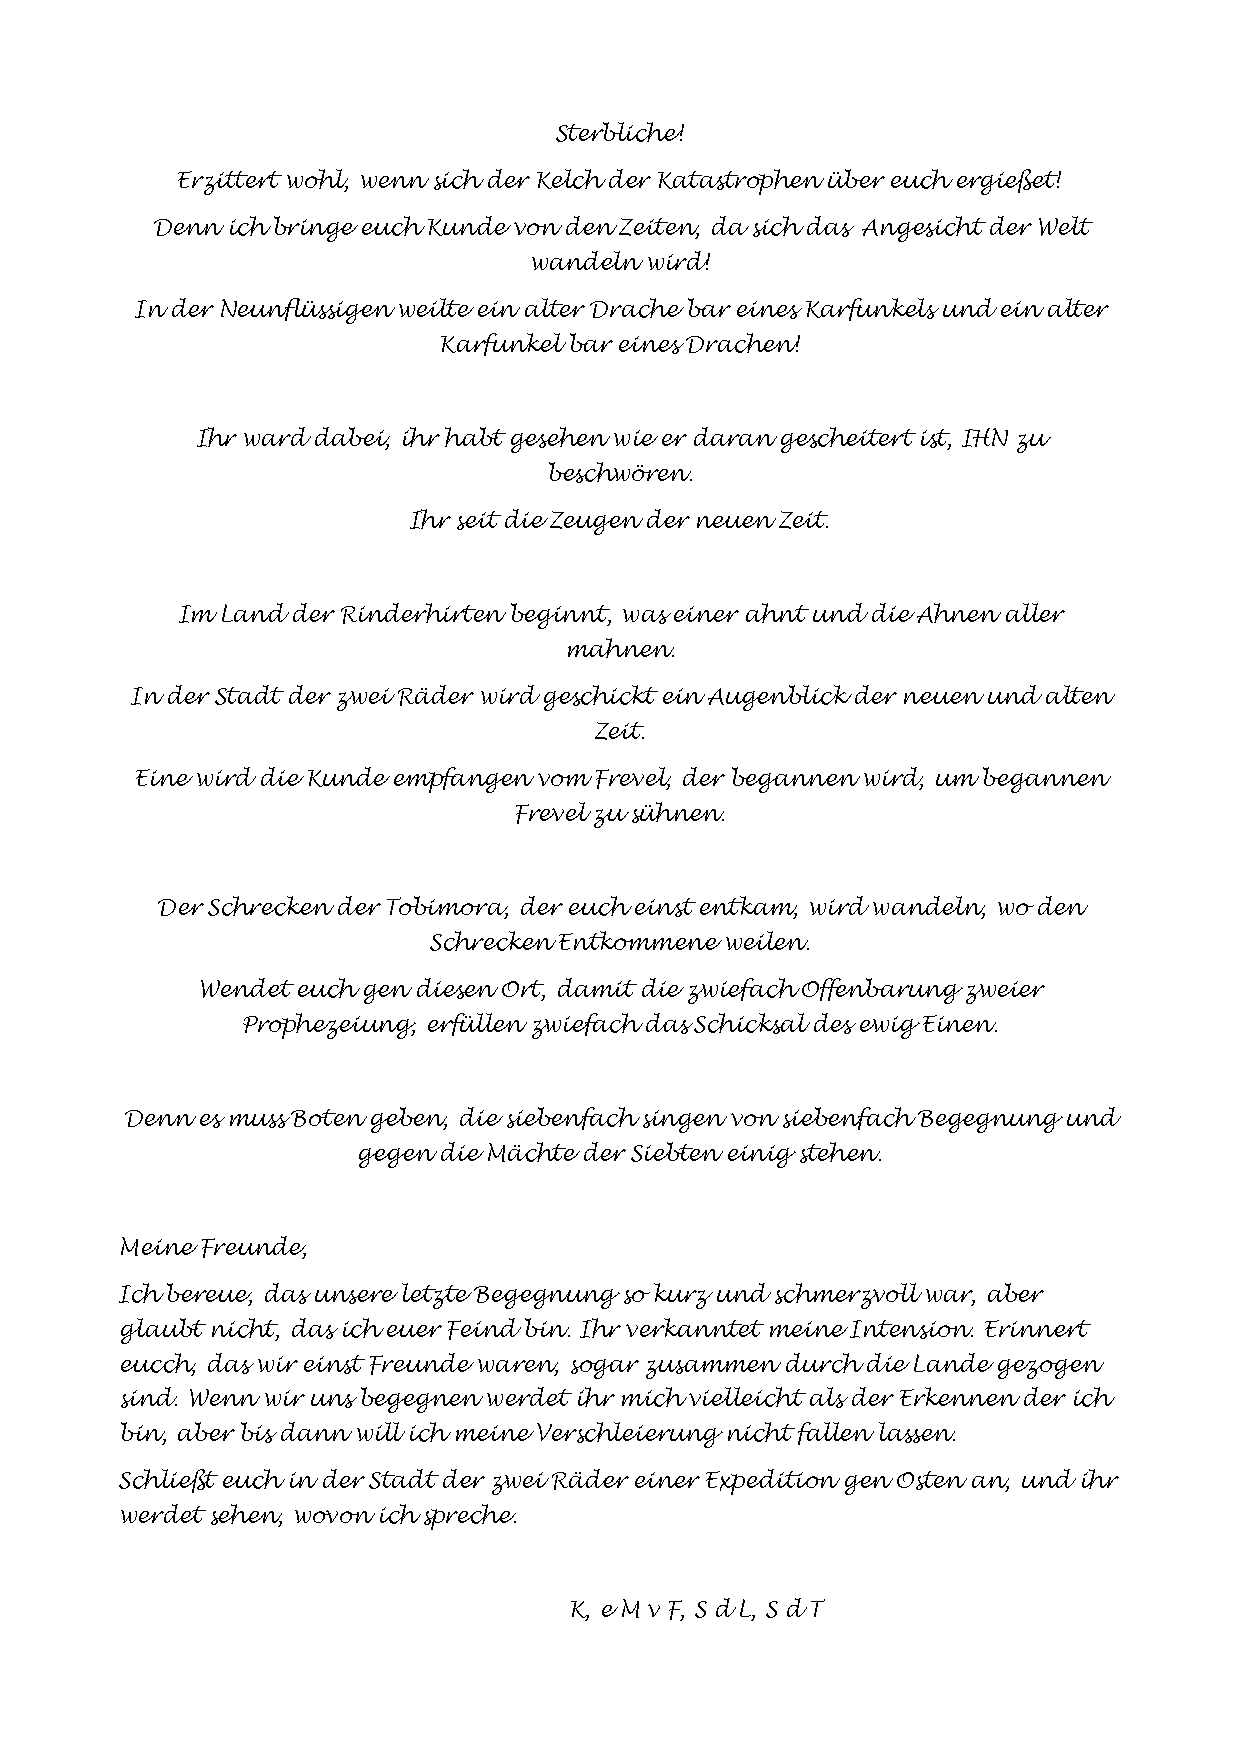
\includepdf[scale=0.9,pages=-]{handouts/part_1/aoe_brief_markhalm.pdf}

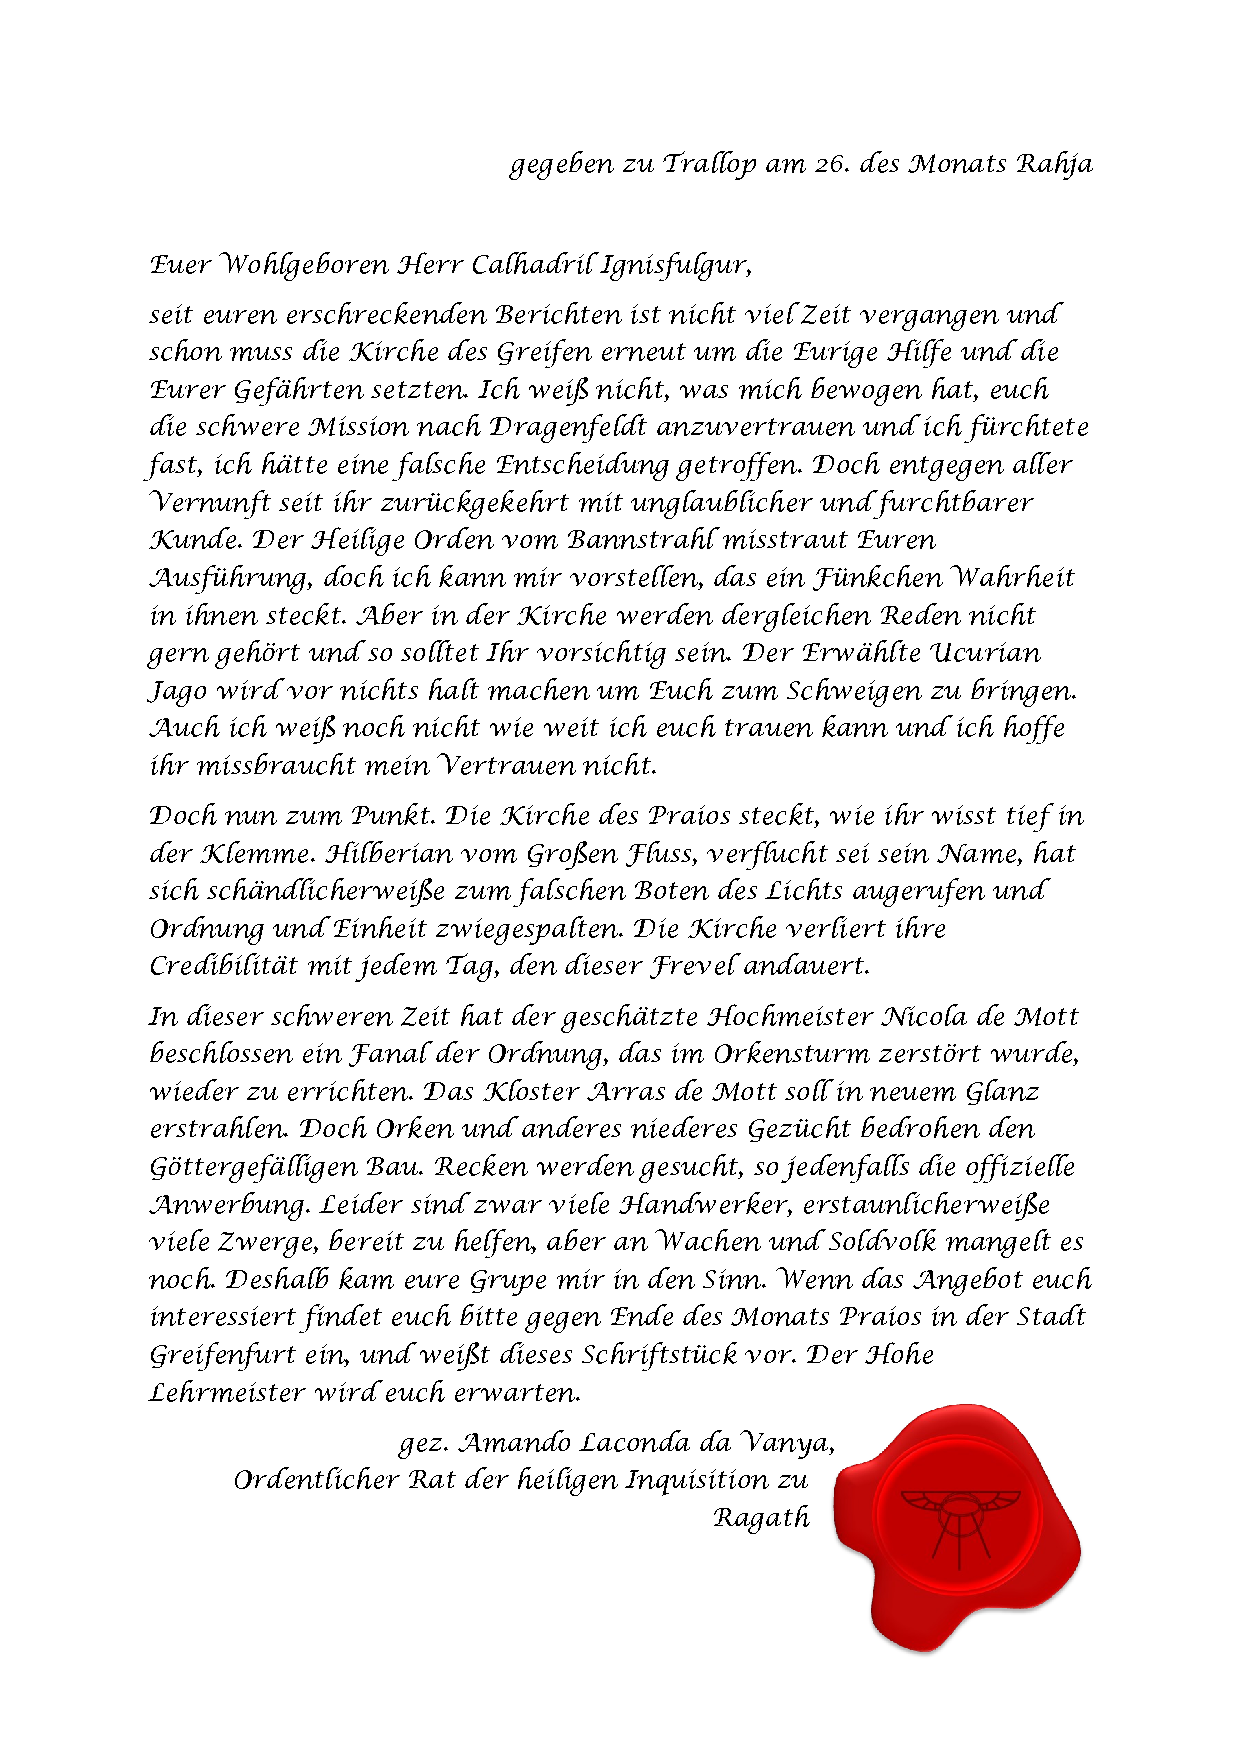
\includepdf[scale=0.9,pages=-]{handouts/part_1/gm_brief_temyr.pdf}

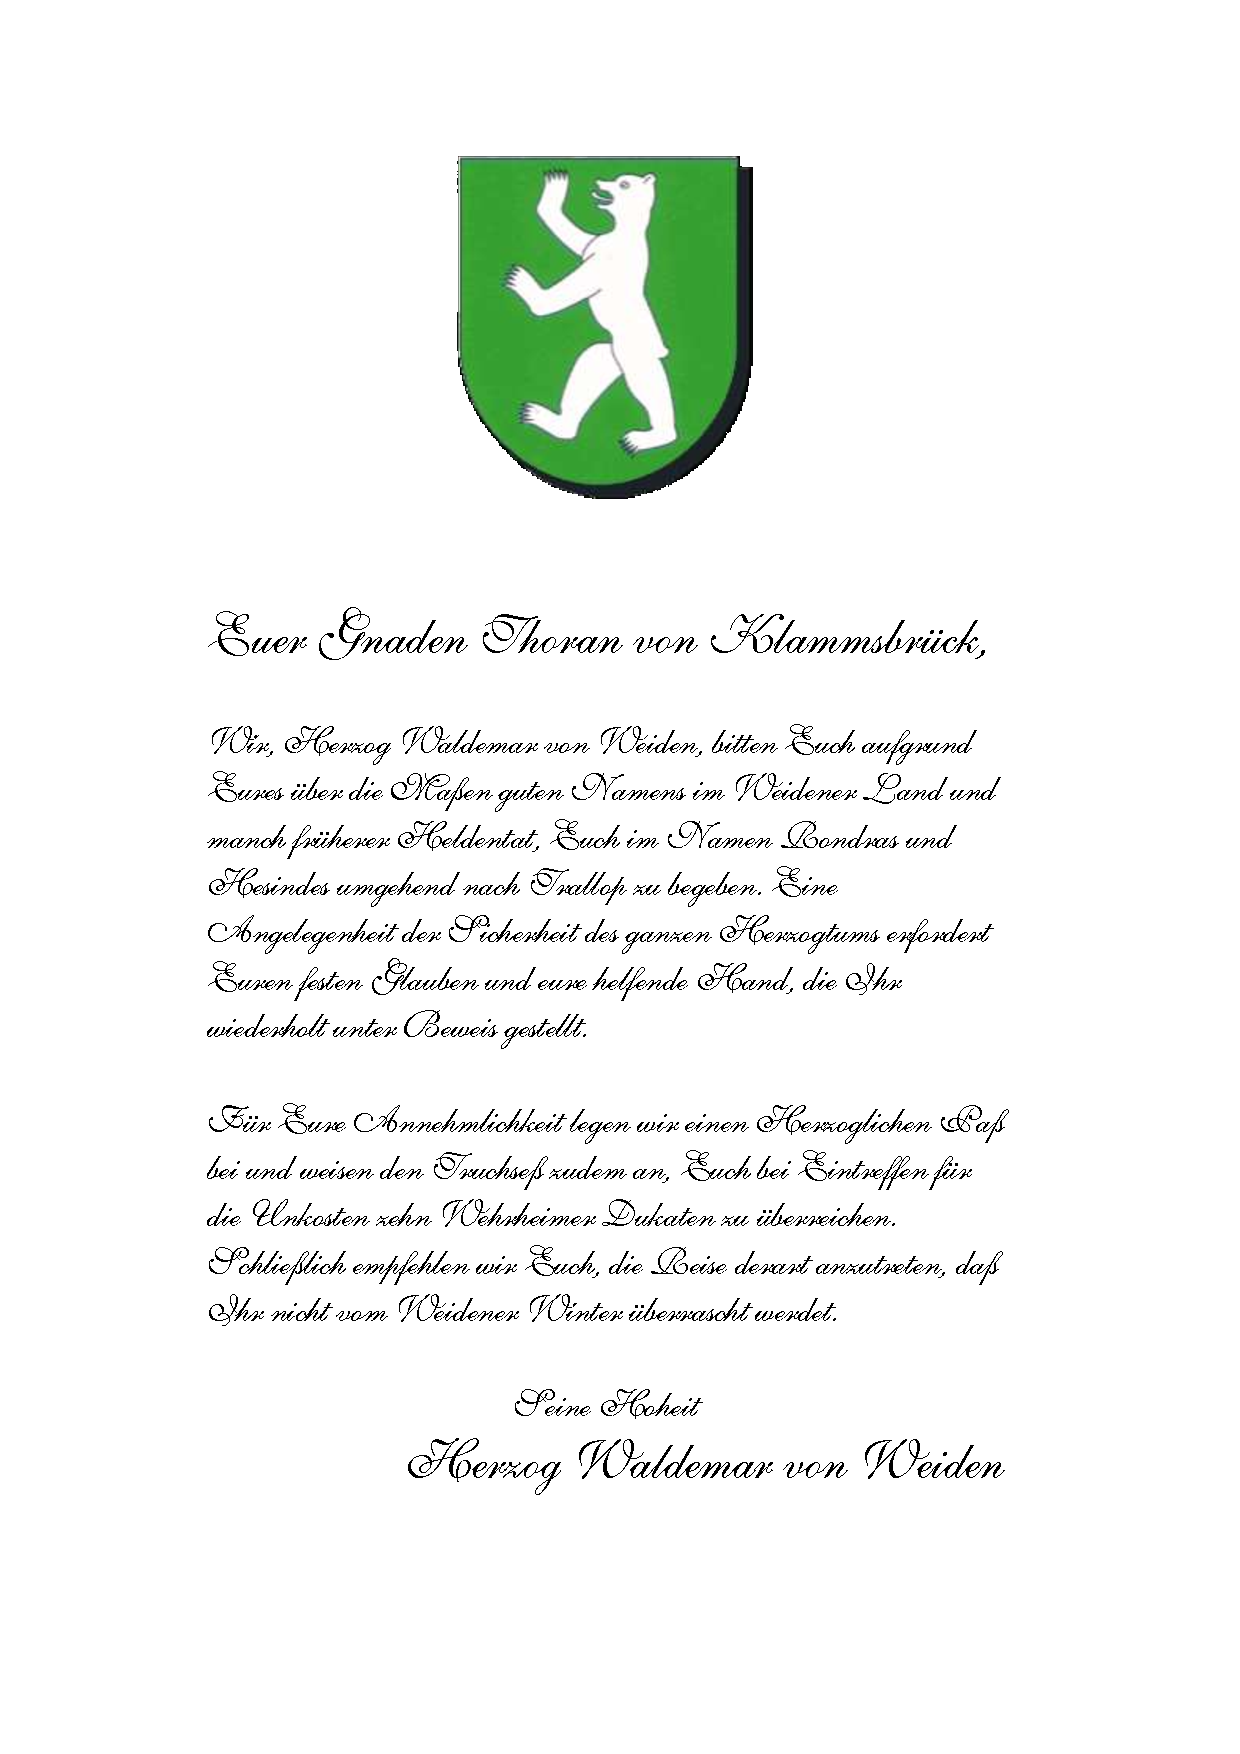
\includepdf[scale=0.9,pages=-]{handouts/part_1/ug_waldemars_brief_Thoran.pdf}

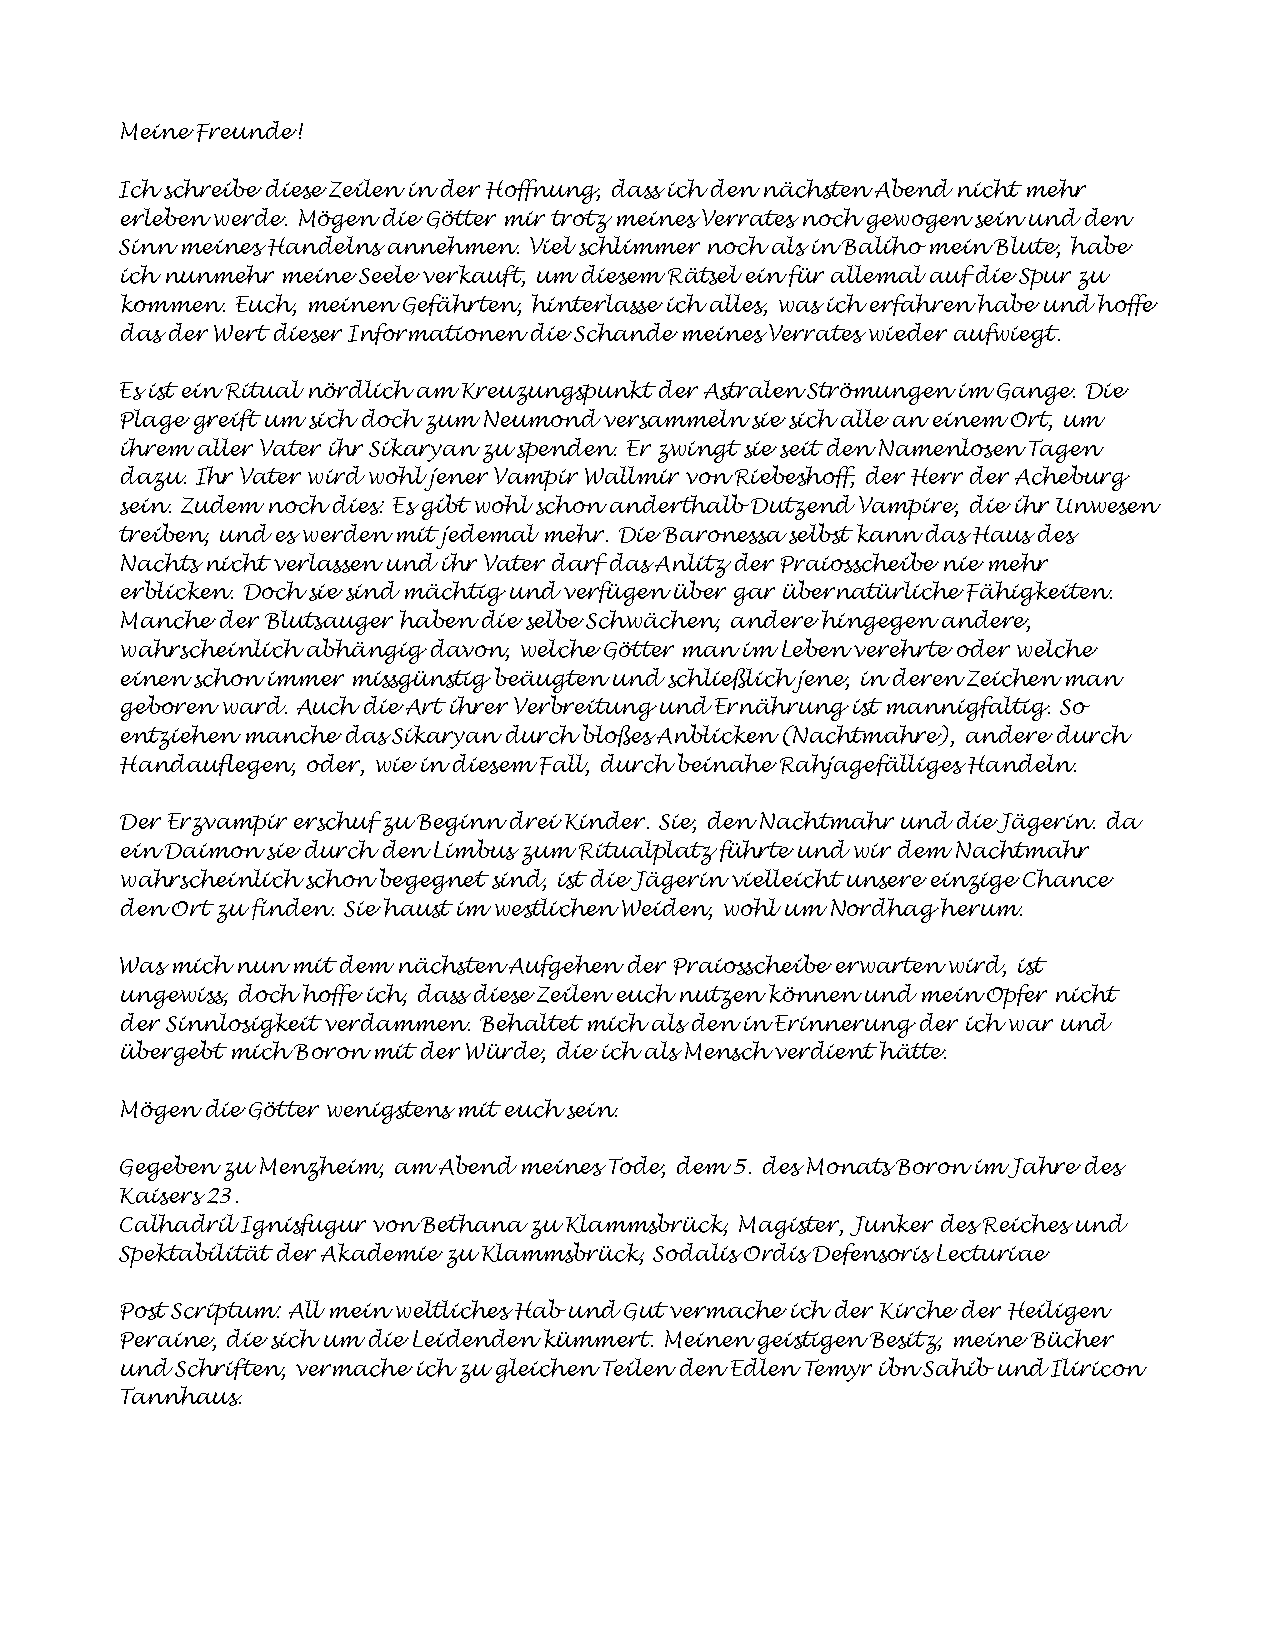
\includepdf[scale=0.9,pages=-]{handouts/part_1/ug_abschied_calhadril.pdf}

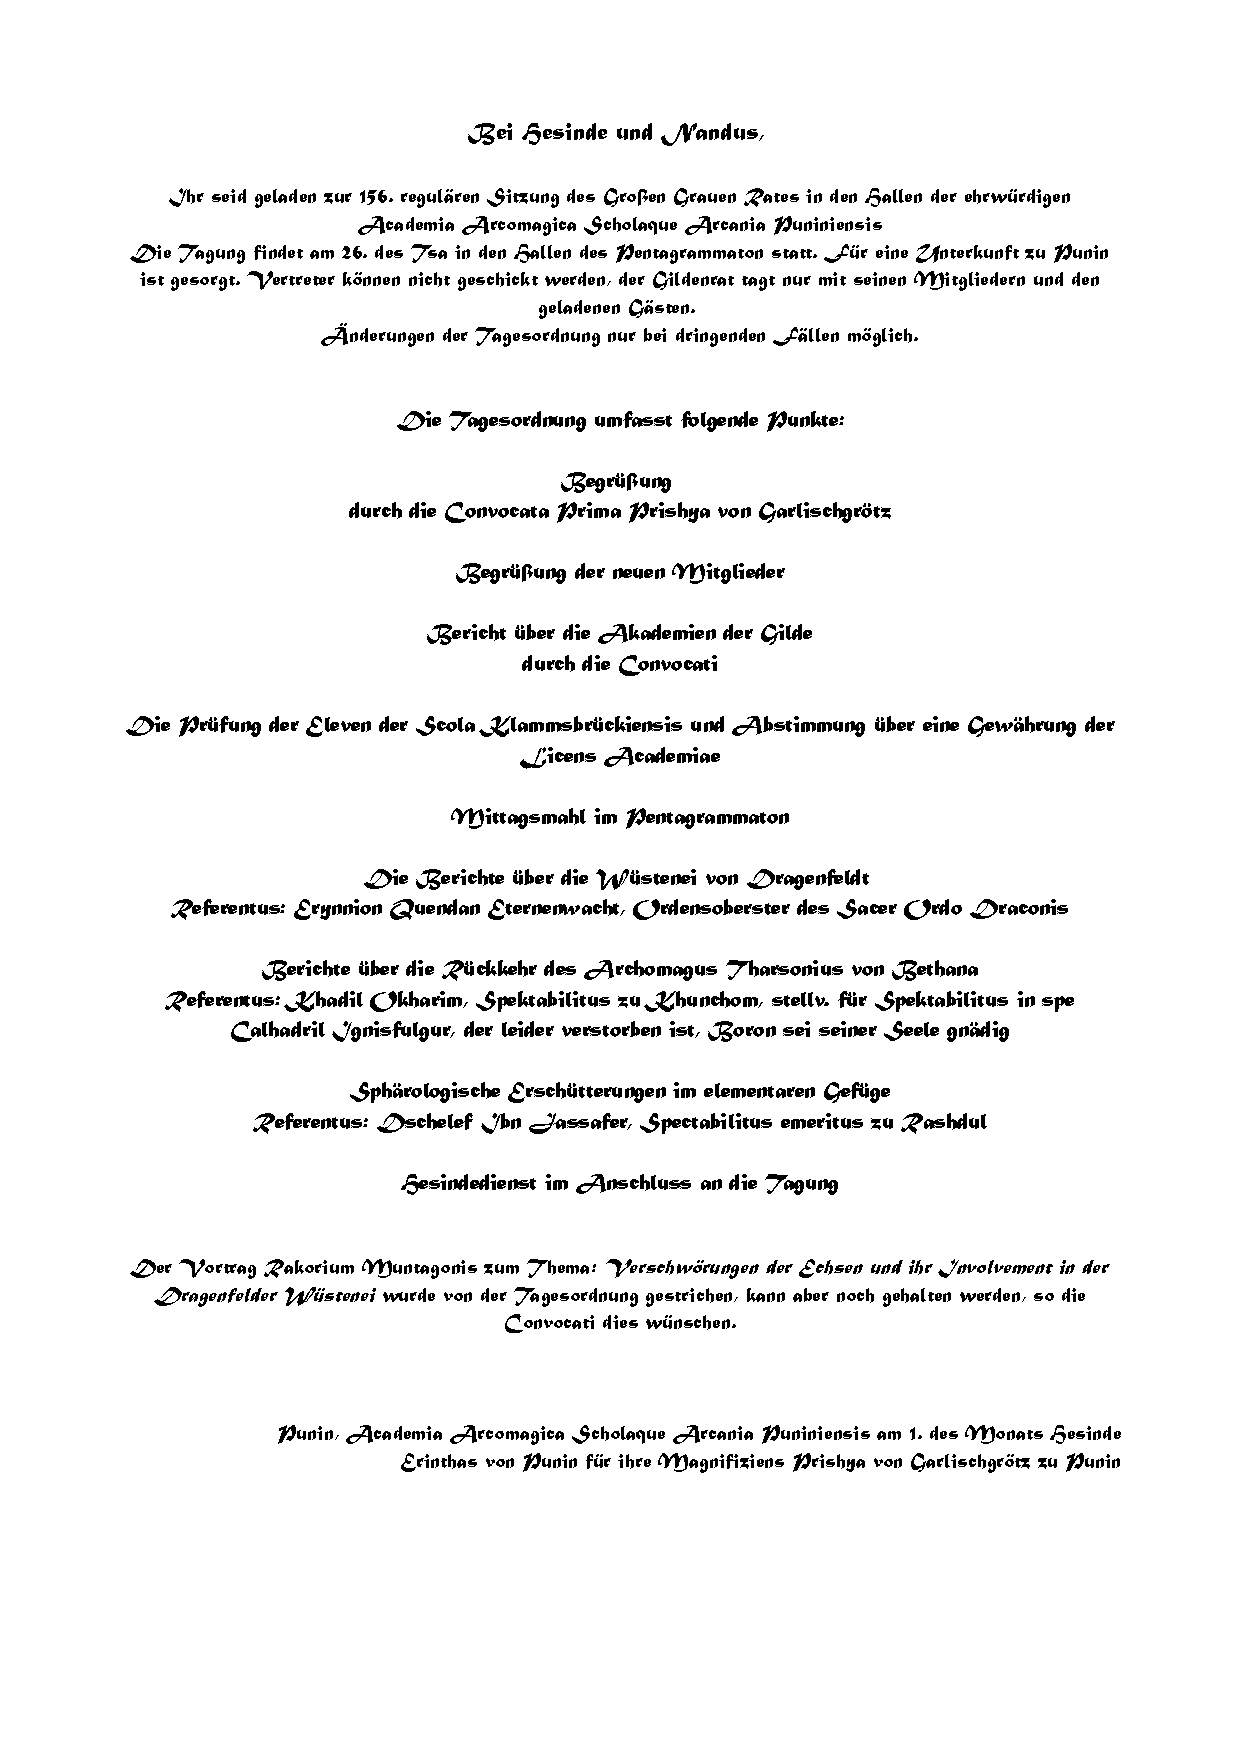
\includepdf[scale=0.9,pages=-]{handouts/part_1/einladung_gildenconvent_ggg.pdf}